\label{sec:experiments}


\begin{figure*}[t]
  \centering
%   \vspace{-0.1cm} 
  \setlength{\abovecaptionskip}{0cm} 
%   \setlength{\belowcaptionskip}{-0.05cm} 
  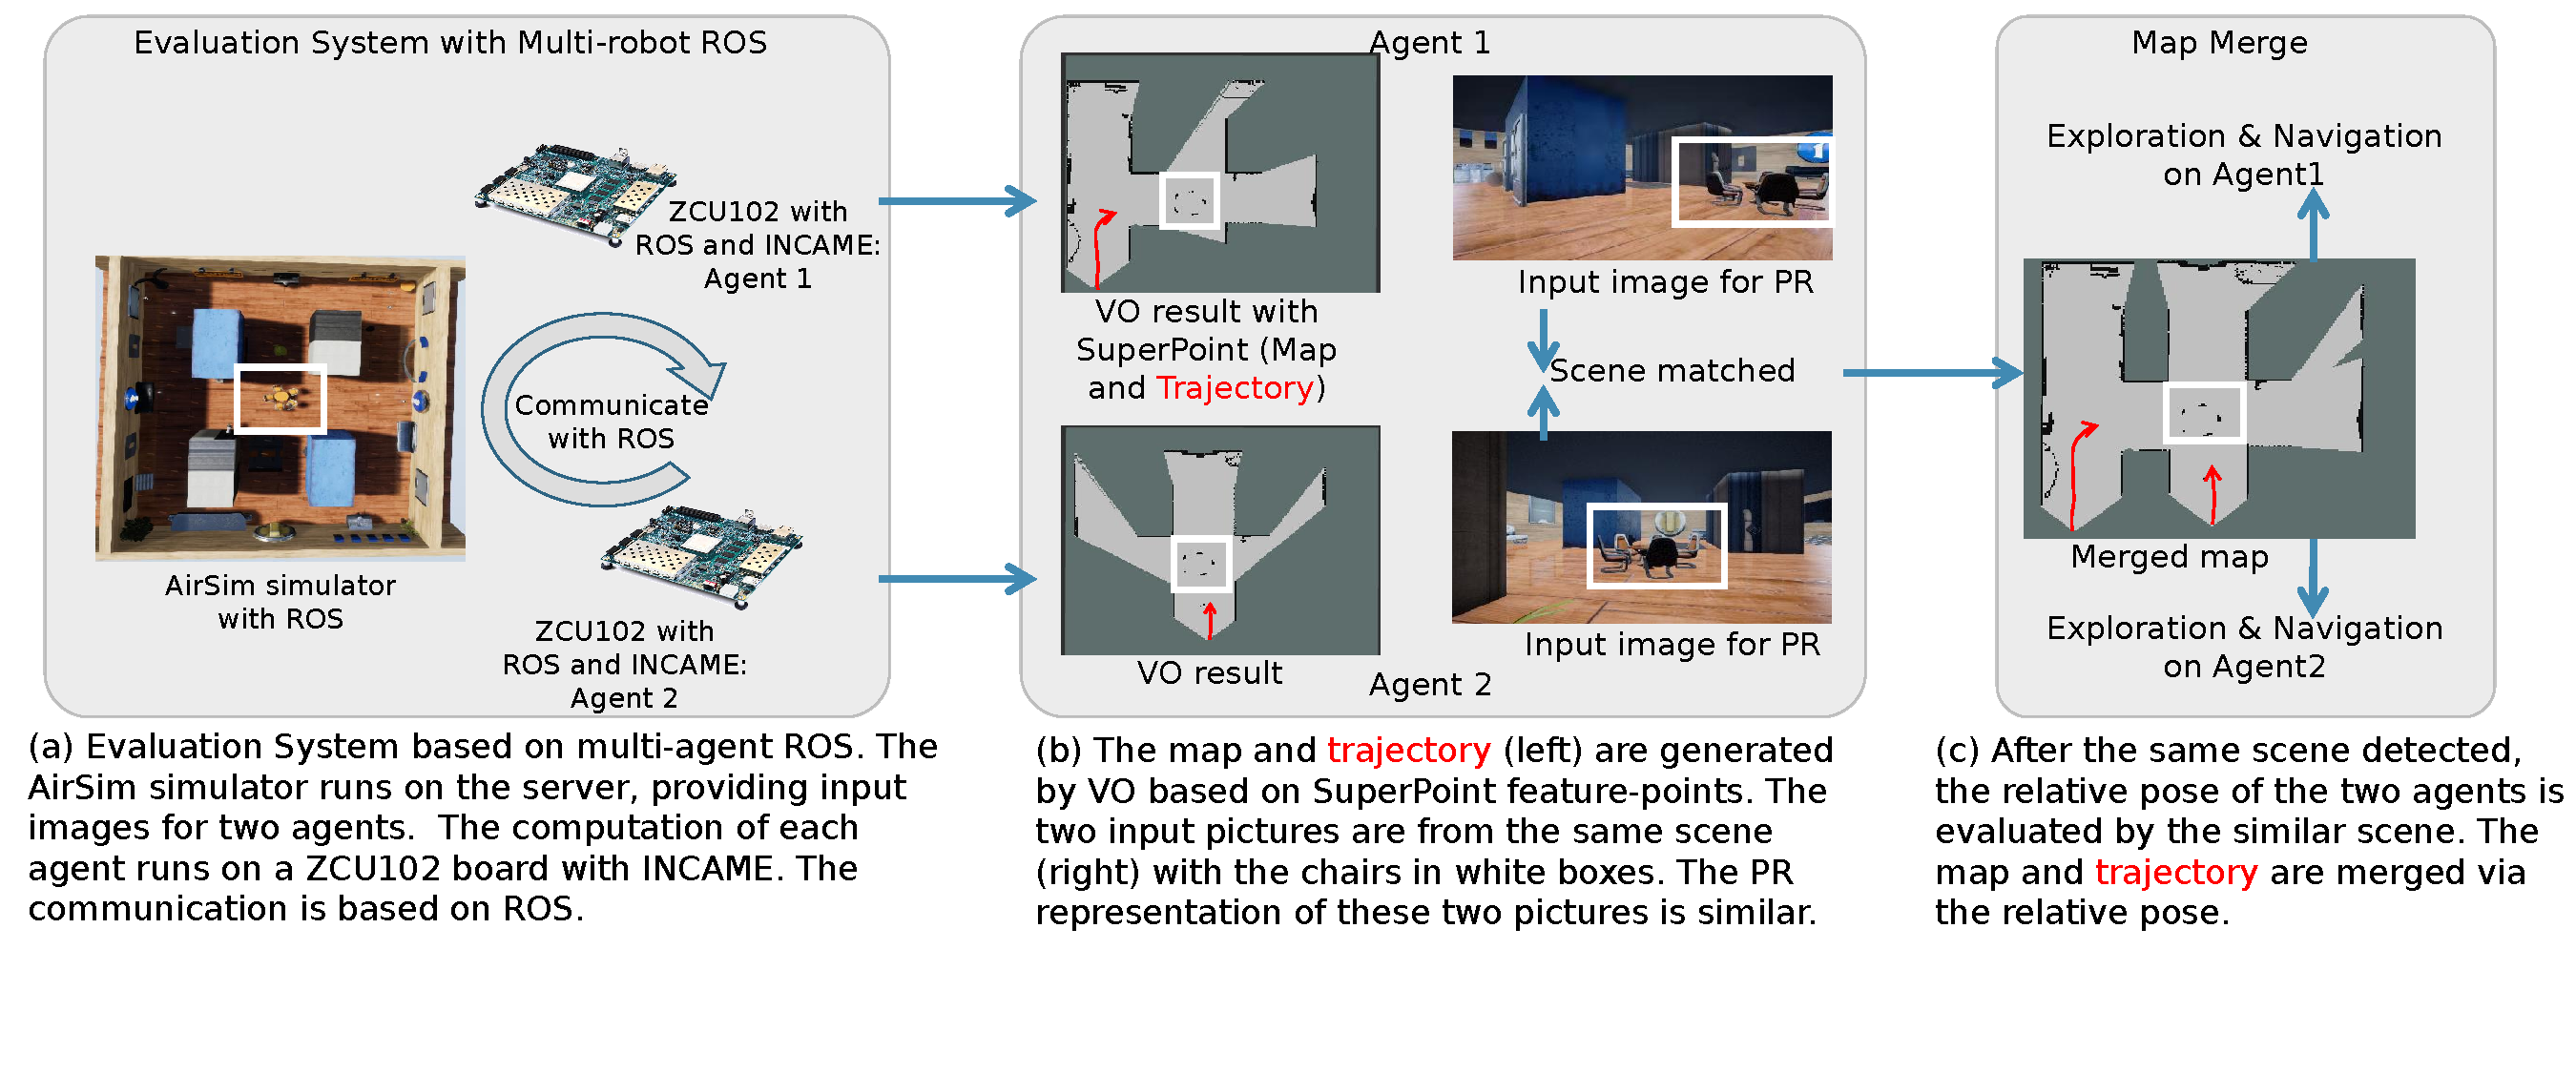
\includegraphics[width=0.99\linewidth]{fig/env.pdf}
  \caption{Multi-robot exploration: environment and results. }
  \label{fig:env}
\end{figure*}


% In this section, the evaluation of the instruction-based-interruption, hardware modules for FE post-processing, and the overall MR-Exploration system are presented and analyzed.



\subsection{ Experiment Setup }

The hardware-in-loop evaluate environment is illustrated in \Cref{fig:env}(a). There is a simulation server providing the simulation environment based on AirSim  ~\cite{shah2018airsim}, which is a high-fidelity visual and physical simulation for autonomous vehicles. The AirSim simulation server provides the camera data for each agent. Two Xilinx ZCU102 boards  ~\cite{zcu102}, with ZU9 MPSoC  ~\cite{MPSoC}, are responsible for the calculation of each agent. 
The components in \Cref{fig:maexp} for each agent are implemented in the ZCU102 board. The implementation of the FE (\textcircled{1} in \Cref{fig:maexp}), SuperPoint ~\cite{detone2018superpoint}), are introduced in former sections. GeM  ~\cite{radenovic2018fine} is used to implement the PR module (\textcircled{2}). GeM is a CNN-based method with ResNet101 \cite{he2016deep} as the backbone, and the post-processing of GeM calculates the 3-norm of the output featuremaps.
The VO module (\textcircled{3}) in the experiment is the PnP  ~\cite{LepetitMoreno-Noguer-EPnP} method, which is widely used in the feature-point based VO. 
% including the open source the ORB-SLAM  ~\cite{Mur-Artal:2017281}. 
The DOpt module (\textcircled{4}) is proposed in  ~\cite{Choudhary:2017e66} and also used in former distributed SLAM system ~\cite{cieslewski2018data}. 
The Map Merging  ~\cite{Andre2014} (\textcircled{5}), Exploration  ~\cite{8202319} (\textcircled{6}), and Navigation  ~\cite{tbd} (\textcircled{7}) in this work are provided by the ROS framework. 

The hardware resources are listed in \Cref{tab:hardware}. The CNN backbone is calculated by the Angel-Eye CNN accelerator ~\cite{guo2017angel} on the FPGA side of ZCU102 (Programmable logic, PL side). The FE post-processing steps run on our proposed accelerators, also on the PL side. The PL side has 2 clock frequencies. The CNN accelerator and the IAU are running at 300MHz. The accelerator for FE post-processing is running at 200MHz. Compared with the CNN accelerator, IAU and FE post-processing use very little hardware resources.

% Table generated by Excel2LaTeX from sheet 'Sheet1'
\begin{table}[t]
  \centering
  \setlength{\abovecaptionskip}{2pt}
  \caption{Hardware consumption of the proposed hardware}
% Table generated by Excel2LaTeX from sheet 'Sheet1'
\begin{tabular}{|c|c|c|c|c|}
  \hline
        & $\# DSP$ & $\# LUT$ & $\# FF$ & $\# BRAM$ \\
  \hline
  On-Board resource &   2520   &  274080      &  548160     & 912 \\
  \hline
  CNN accelerator &   1282   &  74569      &   171416    & 499 \\
  \hline
  IAU &   0   &  2268      &   4633    & 4 \\
  \hline
  FE post-processing & 25      &  17573     &   29115    & 10 \\
  \hline
  \end{tabular}%
  
  \label{tab:hardware}%
\end{table}%


\subsection{Virtual Instruction-based interrupt }

\subsubsection{ Interrupt response latency and extra cost}


We evaluate the latency to respond the interrupt and the performance degradation of different interrupt method. In MR-Exploration, only the low-priority PR task is interruptible, and the interrupt position is unpredictable. GeM  ~\cite{radenovic2018fine} is used to implement the PR module in the experiment.
The CNN backbone of the GeM is ResNet101  ~\cite{he2016deep}, which contains 101 convolution layers. The input shape of the CNN is $480 \times 640 \times 3$. The parallelism of the Angel-Eye is $Para_{height}=8$, $Para_{in}=16$, $Para_{out}=16$, i.e. each CALC instruction processes 8 lines from 16 input channels to 16 output channels. 
% Thus, we randomly selected some interrupt locations inside the PR network.

As shown in \Cref{fig:scatter1024}(a), the latency to respond the interrupt in CPU-like method consists of the time to finish current executing instruction and the data backup time ($t_{latency} = t_1+t_2$) for the on-chip data/weights caches (totally 2.2MB). The latency in layer-by-layer interrupt is the time to finish current layer. The latency of our virtual-instruction-based method is the time to finish current executing instruction and the backup time for the calculated output results. 

The cost of CPU-like interrupt is the data transfer time of all the on-chip caches (totally 2.2MB) to/from DDR ($t_{cost} = t_2+t_4$). The cost of virtual-instruction-based method is only the recovery of the input/weights from DDR to on-chip caches ($t_{cost} = t_4$). There is no extra cost for the layer-by-layer interrupt.

% For a precise evaluation the CNN run time, we record the clock cycles of the beginning and end of each instruction. The time of the interrupt response latency and the total cost in the following evaluation is calculated from the clock cycles and the clock frequence.


We randomly sample 12 positions of the ResNet101 CNN backbone. The interrupt response latency and the extra time cost for different implementation of interrupt at the positions are listed in \Cref{fig:scatter1024}(b).
The CPU-like interrupt consumes the most extra cost ($t_{cost}$). Though the layer-by-layer interrupt consumes no extra time, the latency is much higher than our virtual-instruction-based interrupt. 
This is because the layer-by-layer interrupt need to wait for completion of a layer. The performance at same interrupt position in our proposed virtual interrupt can interrupt inside a layer, with lower latency.


\subsubsection{ Additional data transfer for the virtual instructions. }
% The worst latency of the layer-by-layer interrupt reaches 10 ms, because the interrupt occurs at the beginning of the second layer, which is the most time-consuming layer (10ms). The layer-by-layer interrupt need to wait for the finish of this layer. The performance at same interrupt position in our proposed virtual interrupt is not significantly different from that of other positions. Our method is significantly better than others at worst case. 

The extra virtual instruction number is listed in \Cref{tab:instrnum}. Compared to the normal instruction transfer, the volume of virtual instructions is less than 10\%. The performance degradation brought by the extra virtual instructions is negligible. 
We are here to remind the readers that the processing of the low-priority PR task can be interrupted twice or more. And in that case, the PR task is interrupted by several FE tasks.



% DPU first calculates all channels of the output row before calculating the next rows. As the number of channels increases, the number of weights requiring recovery increases squarely. However, the size of the input data to be restored and the output results to be backed up remains basically the same.


% % Table generated by Excel2LaTeX from sheet 'Sheet2'
% \begin{table}[t]
%   \small
%   \centering
%   \caption{Worst latency different interrupt positions.}
%     % Table generated by Excel2LaTeX from sheet 'Sheet2'
% \begin{tabular}{|c|c|c|c|c|c|}
%   \hline
%         & Backup  & Recovery & CPU-like & layer-by-layer & Virtual Instr. \bigstrut[t]\\
%         & (KB)  & (KB)  &  Latency (ms) & Latency (ms)   & Latency (ms) \bigstrut[b]\\
%   \hline
%   Pose 1 &       &       &       &      &  \bigstrut\\
%   \hline
%   Pose 2 &       &       &       &      &  \bigstrut\\
%   \hline
%   Pose 3 &       &       &       &      &  \bigstrut\\
%   \hline
%   CPU-Like & 4000  & 4000  &     &       & <1 \bigstrut\\
%   \hline
%   Serial & -     & -     &     &   & - \bigstrut\\
%   \hline
%   \end{tabular}%
  
  
%   \label{tab:anywhere}%
% \end{table}%


\begin{figure}[t]
  \centering
%   \vspace{-0.1cm} 
  \setlength{\abovecaptionskip}{0cm} 
%   \setlength{\belowcaptionskip}{-0.05cm} 
  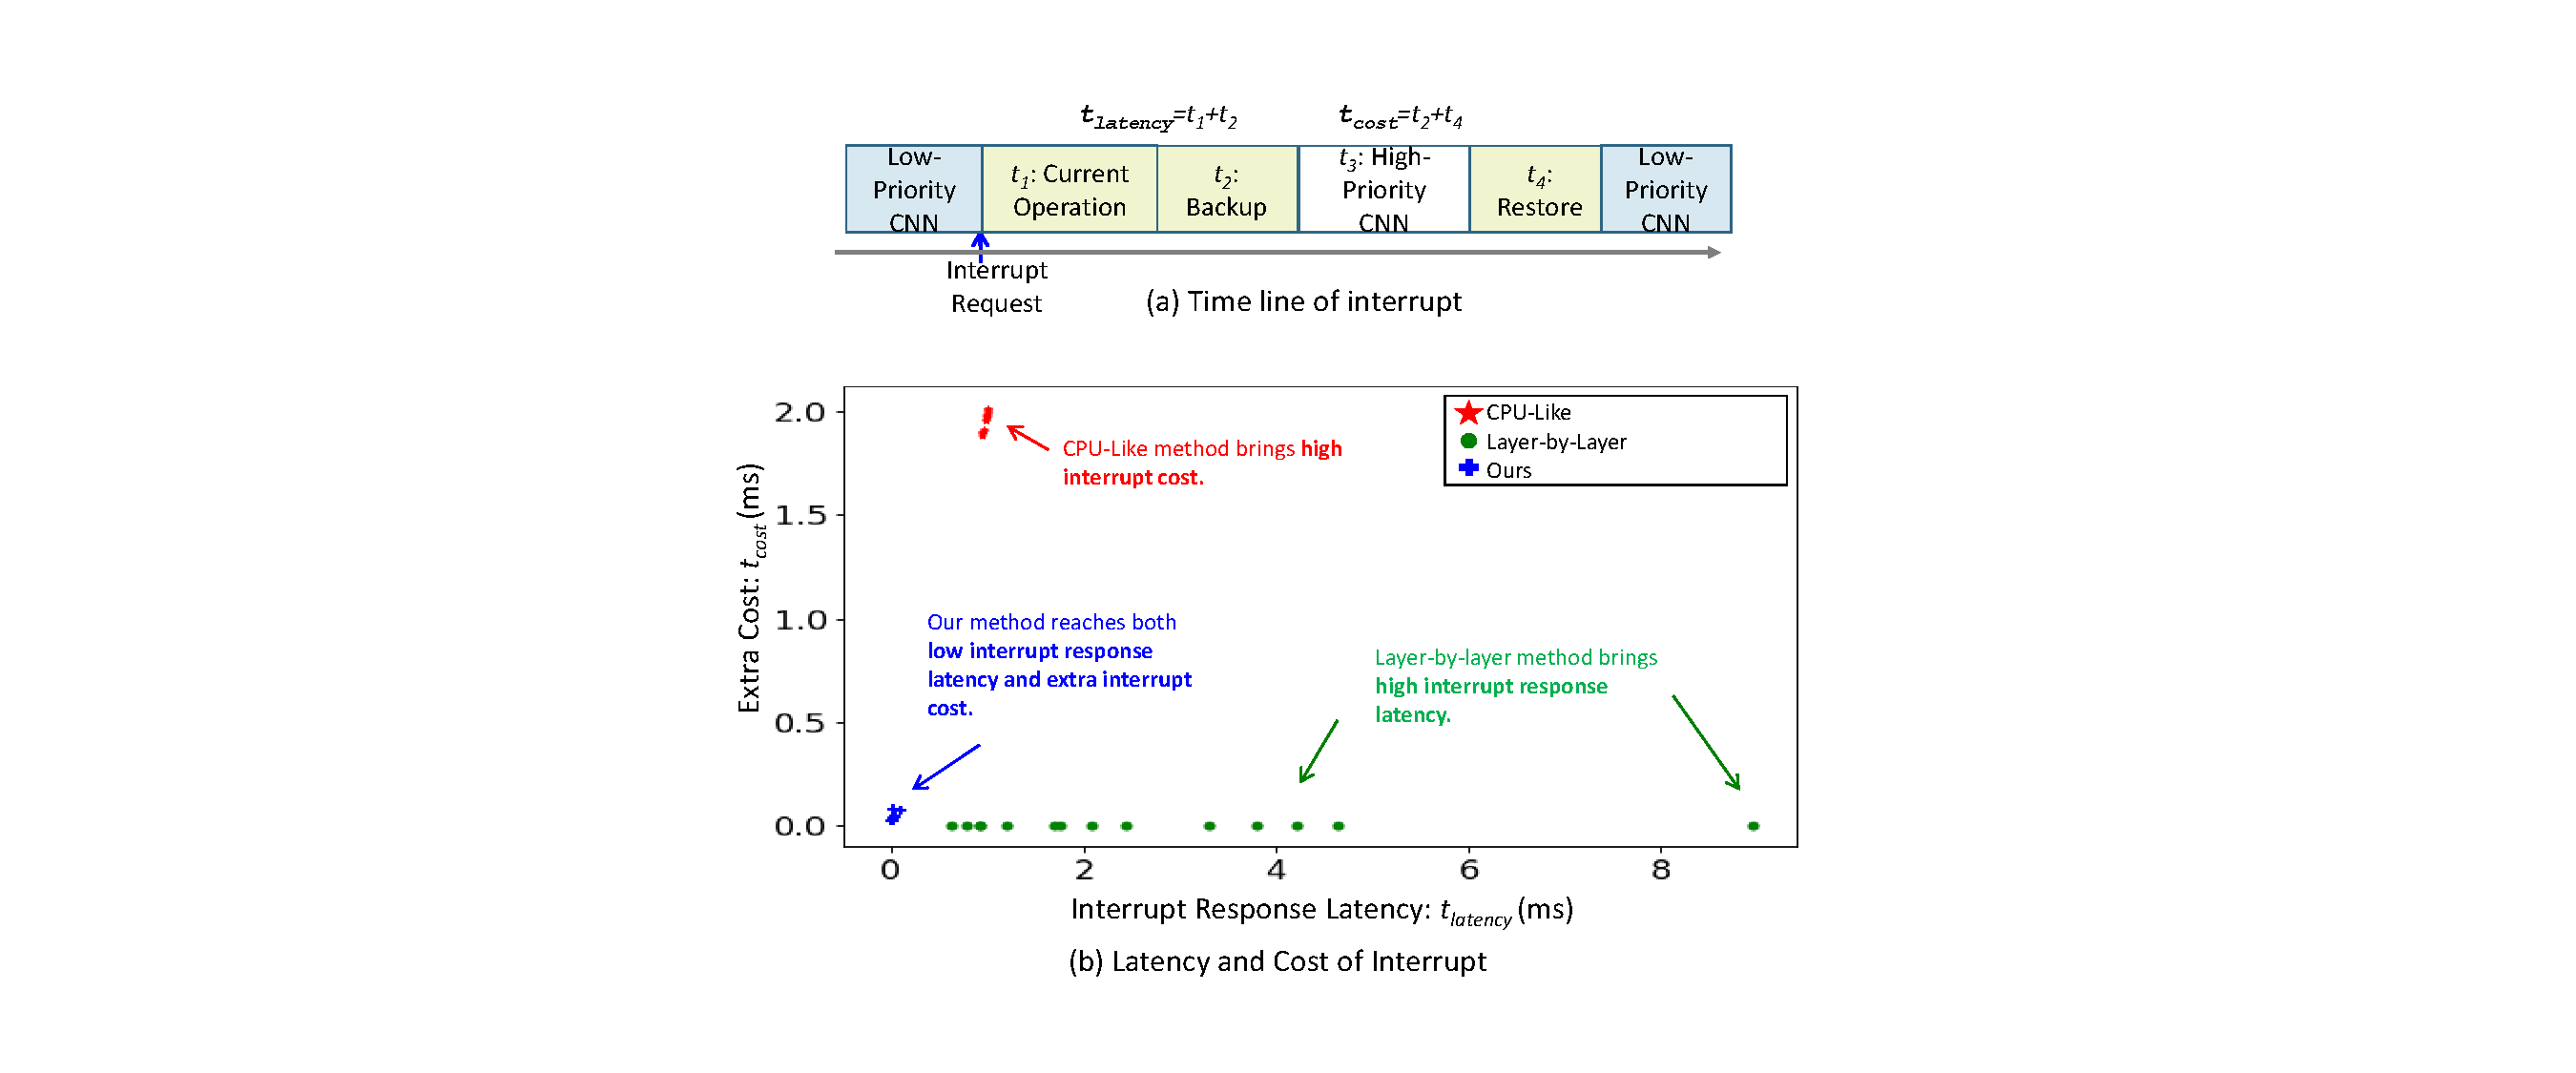
\includegraphics[width=0.99\linewidth]{fig/PRresult.pdf}
  \caption{The interrupt response latency \& extra time cost.}
  \label{fig:scatter1024}
\end{figure}
% Table generated by Excel2LaTeX from sheet 'Sheet2'
\begin{table}[t]
  \small
  \centering
  \setlength{\abovecaptionskip}{2pt}
  \caption{The instruction number of the interruptible PR network (backbone). }
    % Table generated by Excel2LaTeX from sheet 'Sheet2'
\begin{tabular}{|c|c|c|c|c|c|}
  \hline
         & Instr.  & Instr. & Execute \\
        & Number   & volume (MB) & Time (ms) \\
  \hline
  Original ISA   &      364032      & 4.36 & 186.0 \\
  \hline
  VI-ISA   &     400243    & 4.80 & 186.4 \\
  \hline
  \end{tabular}%
  \label{tab:instrnum}%
\end{table}%



% % Table generated by Excel2LaTeX from sheet 'Sheet1'
% \begin{table}[t]
%     \centering
%     \caption{Interrupt after complete results vs Interrupt anywhere}
% % Table generated by Excel2LaTeX from sheet 'Sheet2'
% \begin{tabular}{|c|c|c|c|c|c|}
%   \hline
%   \multicolumn{1}{|c}{} &       & \multicolumn{1}{c|}{Backup } & \multicolumn{1}{c|}{Recovery} & Exe time & Performance \bigstrut[t]\\
%   \multicolumn{1}{|c}{} &       & \multicolumn{1}{c|}{data (KB)} & \multicolumn{1}{c|}{ data (KB)} & (ms)  & Reduce \bigstrut[b]\\
%   \hline
%   \multicolumn{1}{|p{3.315em}|}{Inter } & \multicolumn{1}{p{3.69em}|}{AfterSave} &       &       &       &  \bigstrut\\
%   \cline{2-6}\multicolumn{1}{|p{3.315em}|}{position 1} & Anyware &       &       &       &  \bigstrut\\
%   \hline
%   \multicolumn{1}{|p{3.315em}|}{Inter } & \multicolumn{1}{p{3.69em}|}{AfterSave} &       &       &       &  \bigstrut\\
%   \cline{2-6}\multicolumn{1}{|p{3.315em}|}{ position 2} & Anyware &       &       &       &  \bigstrut\\
%   \hline
%   \multicolumn{1}{|p{3.315em}|}{Inter } & \multicolumn{1}{p{3.69em}|}{AfterSave} &       &       &       &  \bigstrut\\
%   \cline{2-6}\multicolumn{1}{|p{3.315em}|}{position 3} & Anyware &       &       &       &  \bigstrut\\
%   \hline
%   \multicolumn{2}{|p{7.005em}|}{CPU-Like} &       &       &       &  \bigstrut\\
%   \hline
%   \multicolumn{1}{|c}{} &       & \multicolumn{1}{c|}{Instruction} & \multicolumn{1}{c|}{Latency} & Exe time & Performance \bigstrut[t]\\
%   \multicolumn{1}{|c}{} &       & \multicolumn{1}{c|}{ (KB)} & \multicolumn{1}{c|}{(ms)} & (ms)  & Reduce \bigstrut[b]\\
%   \hline
%   \multicolumn{1}{|c|}{No} & \multicolumn{1}{p{3.69em}|}{Origin} &       &       &       & 0 \bigstrut\\
%   \cline{2-6}\multicolumn{1}{|c|}{ Interrupt} & \multicolumn{1}{p{3.69em}|}{After results} &       &       &       &  \bigstrut\\
%   \cline{2-6}      & Anyware &       &       &       &  \bigstrut\\
%   \hline
%   \end{tabular}%
  
%     \label{tab:anywhere}%
%   \end{table}%



% \subsection{ **Place Recognition With the CNN accelerator }

% In this section, we evaluate the accuracy of the PR network on the CNN accelerator with fixed-point number. 

% \begin{figure}[t]
%     \centering
%     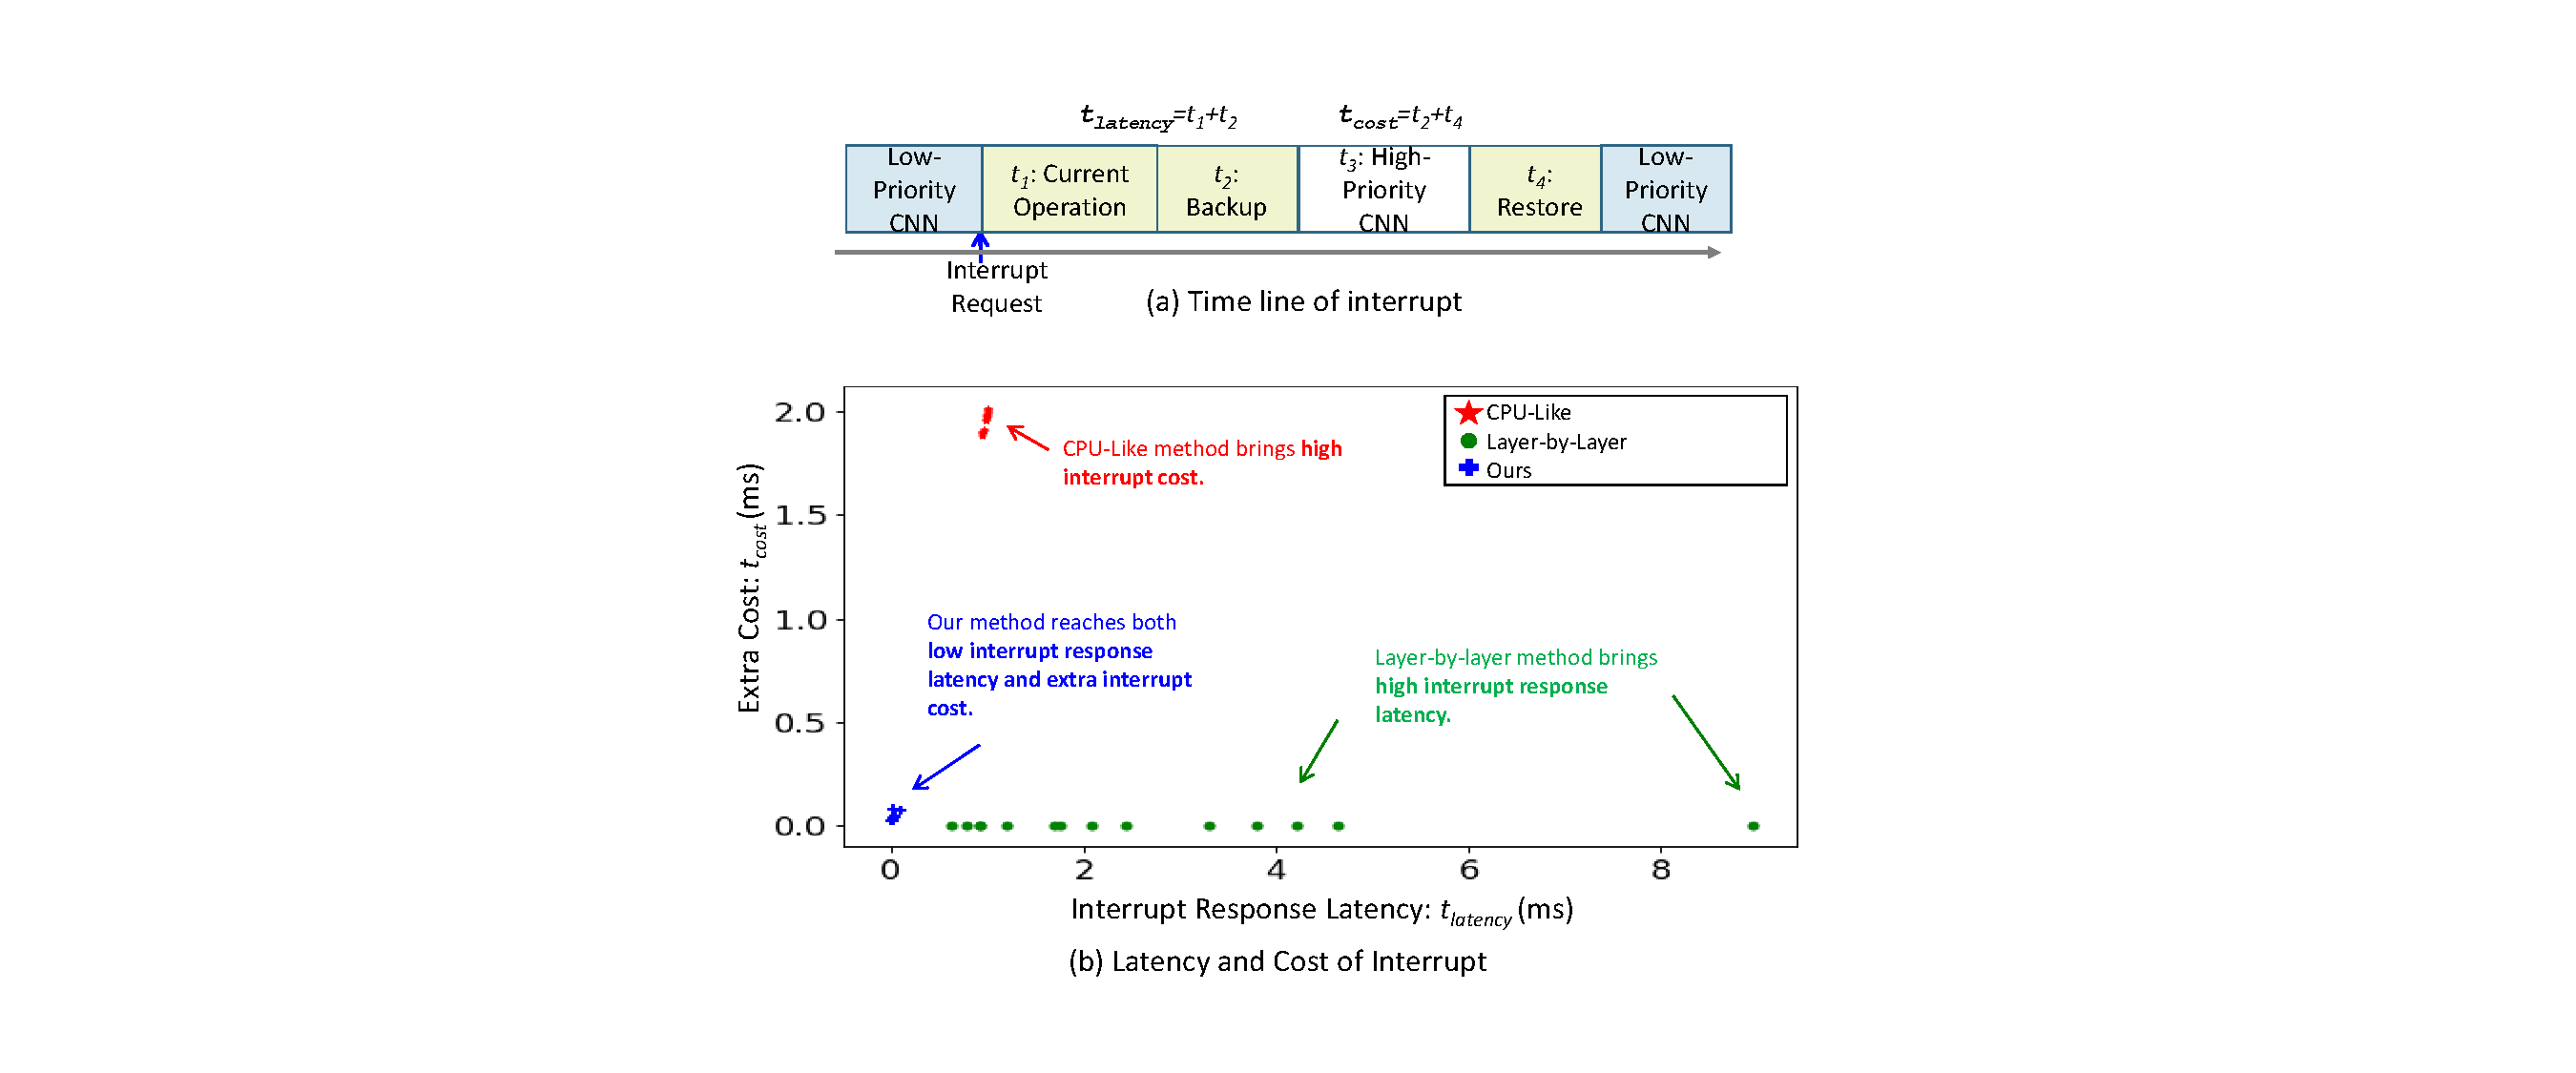
\includegraphics[width=0.8\linewidth]{fig/PRresult.pdf}
%     \caption{Precision-Recall curve on Citycenter dataset}
%     \label{fig:PRcurve}
% \end{figure}

% % We want to prove two things in our experiment. 1) The GeM network used in our work outperforms other networks such as NetVLAD. 2) The quantization of GeM CNN backbone don't bring about much drop in accuracy. 
% We test 3 networks, a) float-point GeM, b) float-point NetVLAD, c) fixed-point GeM on Citycenter dataset [??] and draw the Precision-Recall curve. The result is shown in figure \ref{fig:PRcurve}. It's clear that after quantization, the accuracy slightly reduced and still outperforms the float-point NetVLAD network  ~\cite{arandjelovic2016netvlad}, especially at higher recall, which is used in the MA-Exploration system.

% \begin{figure}[t]
%   \centering
%   \includegraphics[width=0.8\linewidth]{fig/example.eps}
%   \caption{Example of GeM performance.}
%   \label{fig:gem_exp}
% \end{figure}

% Figure \ref{fig:gem_exp} shows an example in our similation environment. Picture 1 and Picture 2 is photoed in the same place and Picture 3 is photoed in another place. The computed similarity of Picture 1 and 2 is 0.8887, apparently larger than the similarity of Picture 2 and 3 (0.8046).

% \subsubsection{efficiency}

% \begin{table}
%     \label{tab:gem_eff}
%     \centering 
%     \caption{running time comparison of each operation in PR}
%     \begin{tabular}{|c|c|c|}
% 				\hline
%               & CPU & CPU+FPGA \\
%         \hline
%            &   48 ms &   42 ms \\
% 			  \hline
%     \end{tabular}
%   \end{table}

% As illustrated in section \ref{sec:hardsoftcodesign}, we do optimization on GeM backend processing, i.e., the GeM pooling layer. We compare running time before and after optimization, and the result is shown in table \ref{tab:gem_eff}. After optimization, the total time reduces by 12.5\%.


\subsection{ FE Evaluation }

We evaluate the performance of the SuperPoint network in VO on the $TUM$ dataset ~\cite{sturm12iros}. We evaluate SuperPoint against two well-known handcrafted FE systems: SIFT ~\cite{Lowe-478} and ORB ~\cite{Mur-Artal:2017281}. 
We also evaluate the performance after optimization. 
We extract a maximum of 200 feature-points at a $480\times640$ input resolution. 
We perform nearest neighbor matching from descriptors in adjacent frames with a maximum allowable distance $d_m$. $d_m$ is not the same in three FE systems because these three descriptors are different. In PS side, we use an OpenCV implementation (solvePnP()) with all the matches to compute the transform matrix  ~\cite{LepetitMoreno-Noguer-EPnP}, and use Bundle Adjustment (BA) to optimize results  ~\cite{TriggsMclauchlan-Bundle-Adjustment}. 
% All the computation of this experiment is all done on the CPU except CNN of SuperPoint. 

Results are shown in \Cref{tab:VO}. In terms of accuracy, SuperPoint outperforms ORB and SIFT. Our optimizations, including fixed-point quantization, and post-processing acceleration, do not introduce a large loss of accuracy. 
% In terms of calculation speed, SuperPoint takes less time than Sift, and is equivalent to ORB. 
% After optimization, the running speed of SuperPoint is increased by $4\times$, making real-time processing possible.

\begin{table}[t]
  \centering
  \setlength{\abovecaptionskip}{2pt}
  \caption{Running time comparison of each FE operation}
    \begin{threeparttable}
% Table generated by Excel2LaTeX from sheet 'Sheet2'
\begin{tabular}{|c|c|c|c|c|c|}
  \hline
             &CNN$^*$ &    Softmax &        NMS &       Rank &  Norm \\
  \hline
         CPU & \multirow{2}{*}{24ms} &      31ms &       27ms &       0.97ms &       42ms \\
  \cline{1-1} \cline{3-6}
    Ours & \multirow{2}{*}{} &    1.97ms &      0.7ms &     0.12ms &     1.44ms \\
  \hline
  \end{tabular} 
  \small
\begin{tablenotes}
   \item[*] CNN backbone runs on the accelerator.  
\end{tablenotes}
    \end{threeparttable}
  
  \label{tab:optimization}%
\end{table}%

We compare the running time of each operation in SuperPoint post-processing before and after the optimization. Results are shown in \Cref{tab:optimization}. The running time of post-processing is reduced by more than $20\times$. There is a certain gap between the experimental results of the acceleration effect and the theoretical derivation in \Cref{subsec:FEopt}. The possible reason is that the CPU needs time to schedule the FPGA accelerator.

\begin{table}[t]
  \centering
  \setlength{\abovecaptionskip}{2pt} 
  \caption{ Accuracy and running time results on the TUM ~\cite{sturm12iros} dataset  }
  \footnotesize
  \begin{threeparttable}
% Table generated by Excel2LaTeX from sheet 'Sheet2'
\begin{tabular}{|c|c|c|c|} 
  \hline
        & RPE$^2$(m/s) & ATE$^3$(m)  & Running time(ms) \bigstrut\\
  \hline
  SIFT  ~\cite{Lowe-478}  & 0.0319  & 0.4219 & 2397  \bigstrut\\
  \hline
  ORB  ~\cite{Mur-Artal:2017281}  & 0.0577  & 0.6105 & 229  \bigstrut\\
  \hline
  Original SuperPoint  ~\cite{detone2018superpoint} & 0.0280  & 0.3671 & 259  \bigstrut\\
  \hline
  Our Fixed SuperPoint  & 0.0283  & 0.3976 & 59  \bigstrut\\
  \hline
  \end{tabular}%
  

\begin{tablenotes}
  \item[1] RPE is the mean Relative Pose Error to indicate the translational drift per second. The less, the better.
  \item[2] ATE is the root mean square Absolute Trajectory Error to indicate the translational drift of the entire trajectory. The less, the better.
\end{tablenotes}
    \end{threeparttable}
  \label{tab:VO}%
\end{table}%

% \vspace*{-2mm}
\subsection{ ROS based MR-Exploration }

The results of the Multi-Robot Exploration based on INCAME is shown in \Cref{fig:env}. The space in the AirSim~\cite{shah2018airsim} for the robots to explore is shown in \Cref{fig:env}(a). It is a simple rectangle area with four different pillars, and some chairs at the center (in the white box).  \Cref{fig:env}(b) shows how PR works for map merging. The FE and VO of each agent produce the local map and trajectory on each ZCU102 board. When the PR threads on different agents find out a similar scene, the relative pose of the two agents at the similar scene is calculated. The map and the trajectory is merged with the calculated relative pose, as shown in \Cref{fig:env}(c).

In this example, the FE and PR are both executed on the same Angel-Eye accelerator. The frequency of the input camera is 20fps, and each input frame is fed to the FE, and FE module would take up accelerator. While the CPU process VO with the feature-points from FE, the accelerator can switch to process the low-priority PR task. Because the executing time of VO varies, the time to finish a PR task is different. In this example, the time from the beginning of a PR to its end is 320$\sim$500 ms. Thus, the PR process one key frame every 7$\sim$10 input frames.